\chapter{Finite-state automaton}
\section{Finite-state automaton over finite inputs}

\begin{definition}[Deterministic finite-state automaton]
    A \textbf{deterministic finite-state automaton} (DFA) is a $5$-tuple
    \[ (Q, \Sigma, \delta, q_0, F) \]
    where
    \begin{enumerate}
        \item $Q$ is a finite set of states;
        \item $\Sigma$ is a finite alphabet;
        \item $\delta: Q \times \Sigma \to Q$ is a transition function;
        \item $q_0 \in Q$ is a start state; and
        \item $F \subset Q$ is the set of accept states.
    \end{enumerate}
\end{definition}

\begin{definition}[]
    Let $M = (Q, \Sigma, \delta, q_0, F)$ be a DFA and
    $w = (w_1, w_2, \ldots, w_n)$ be a word over $\Sigma$.
    We say $M$ \textbf{accepts} $w$ if there is a sequence of states
    $(r_0, r_1, r_2, \ldots, r_n)$
    such that
    \begin{enumerate}
        \item $r_0 = q_0$;
        \item $\delta(r_i, w_{i + 1}) = r_{i + 1}$
            for all $i \in \{0, \ldots, n - 1\}$; and
        \item $r_n \in F$.
    \end{enumerate}
\end{definition}

\begin{figure}
    \centering
    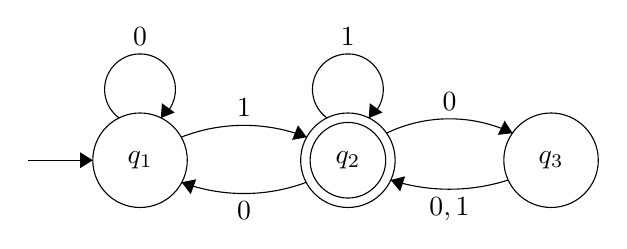
\begin{tikzpicture}[scale=0.2]
        \tikzstyle{every node}+=[inner sep=0pt]
        \draw [black] (22.6,-18.5) circle (3);
        \draw (22.6,-18.5) node {$q_1$};
        \draw [black] (35.8,-18.5) circle (3);
        \draw (35.8,-18.5) node {$q_2$};
        \draw [black] (35.8,-18.5) circle (2.4);
        \draw [black] (48.7,-18.5) circle (3);
        \draw (48.7,-18.5) node {$q_3$};
        \draw [black] (15.5,-18.5) -- (19.6,-18.5);
        \fill [black] (19.6,-18.5) -- (18.8,-18) -- (18.8,-19);
        \draw [black] (21.277,-15.82) arc (234:-54:2.25);
        \draw (22.6,-11.25) node [above] {$0$};
        \fill [black] (23.92,-15.82) -- (24.8,-15.47) -- (23.99,-14.88);
        \draw [black] (25.209,-17.038) arc (111.40762:68.59238:10.935);
        \fill [black] (33.19,-17.04) -- (32.63,-16.28) -- (32.26,-17.21);
        \draw (29.2,-15.78) node [above] {$1$};
        \draw [black] (33.158,-19.903) arc (-69.5919:-110.4081:11.352);
        \fill [black] (25.24,-19.9) -- (25.82,-20.65) -- (26.17,-19.71);
        \draw (29.2,-21.12) node [below] {$0$};
        \draw [black] (34.477,-15.82) arc (234:-54:2.25);
        \draw (35.8,-11.25) node [above] {$1$};
        \fill [black] (37.12,-15.82) -- (38,-15.47) -- (37.19,-14.88);
        \draw [black] (38.245,-16.784) arc (115.73775:64.26225:9.223);
        \fill [black] (46.26,-16.78) -- (45.75,-15.99) -- (45.32,-16.89);
        \draw (42.25,-15.37) node [above] {$0$};
        \draw [black] (45.984,-19.756) arc (-72.20802:-107.79198:12.22);
        \fill [black] (38.52,-19.76) -- (39.12,-20.48) -- (39.43,-19.52);
        \draw (42.25,-20.84) node [below] {$0,1$};
    \end{tikzpicture}
    \caption{A finite-state automaton.}
    \label{fig:dfa-1}
\end{figure}

\begin{example}
    \hfill 
    \begin{enumerate}
        \item 
            The diagram shown Figure \ref{fig:dfa-1} 
            is an example of a DFA.
            This automaton accepts $0100$, but would reject $1010$.
    
        \item The DFA shown in Figure 
            \ref{fig:dfa-2} accepts all 
            binary strings ending in $1$.
    \end{enumerate}
\end{example}

\begin{definition}[]
    Let $M$ be a DFA and $L$ be a formal language.
    We say $M$ \textbf{recognises} $L$ if
    \[ L = \{ w : M \;\text{accepts}\; w \}. \]
\end{definition}

\begin{definition}[Regular language]
    Let $L$ be a formal language.
    We say that $L$ is \textbf{regular}
    if there exists some DFA $M$
    such that $M$ recognises $L$.
\end{definition}

\begin{figure}
    \centering
    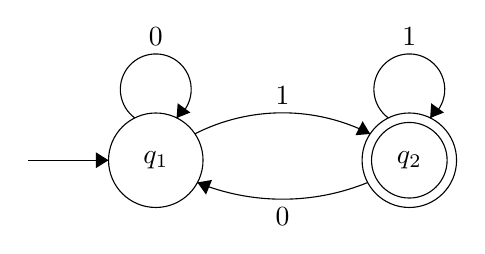
\begin{tikzpicture}[scale=0.2]
        \tikzstyle{every node}+=[inner sep=0pt]
        \draw [black] (25.2,-19.4) circle (3);
        \draw (25.2,-19.4) node {$q_1$};
        \draw [black] (41.3,-19.4) circle (3);
        \draw (41.3,-19.4) node {$q_2$};
        \draw [black] (41.3,-19.4) circle (2.4);
        \draw [black] (17.1,-19.4) -- (22.2,-19.4);
        \fill [black] (22.2,-19.4) -- (21.4,-18.9) -- (21.4,-19.9);
        \draw [black] (23.877,-16.72) arc (234:-54:2.25);
        \draw (25.2,-12.15) node [above] {$0$};
        \fill [black] (26.52,-16.72) -- (27.4,-16.37) -- (26.59,-15.78);
        \draw [black] (27.68,-17.726) arc (117.01458:62.98542:12.262);
        \fill [black] (38.82,-17.73) -- (38.33,-16.92) -- (37.88,-17.81);
        \draw (33.25,-15.89) node [above] {$1$};
        \draw [black] (38.66,-20.814) arc (-67.82872:-112.17128:14.336);
        \fill [black] (27.84,-20.81) -- (28.39,-21.58) -- (28.77,-20.65);
        \draw (33.25,-22.37) node [below] {$0$};
        \draw [black] (39.977,-16.72) arc (234:-54:2.25);
        \draw (41.3,-12.15) node [above] {$1$};
        \fill [black] (42.62,-16.72) -- (43.5,-16.37) -- (42.69,-15.78);
    \end{tikzpicture}
    \caption{A finite-state automaton that accepts strings ending in $1$.}
    \label{fig:dfa-2}
\end{figure}

\begin{proposition}[]
    Let $\Sigma$ be a finite alphabet
    and let $K$ and $L$ be regular languages.
    Then the following are also regular languages:
    \begin{enumerate}
        \item (union)         $K \cup      L$;
        \item (intersection)  $K \cap      L$;
        \item (difference)    $K \setminus L$;
        \item (complement)    $  \overline L       = \Sigma \setminus L$;
        \item (concatenation) $K           L       = \{kl  : k \in K, l \in L\}$; and
        \item (Kleene star)   $            L^\star = \{l^n : n \in \Z_{\geq 0}\}$.
    \end{enumerate}
\end{proposition}

We can use \emph{regular expressions} to 
describe regular languages.

\begin{definition}[Regular expression]
    Let $\Sigma$ be a finite alphabet.
    Then the following constants are defined as \textbf{regular expressions}:
    \begin{enumerate}
        \item (empty set)         $\varnothing$ denoting the empty set;
        \item (empty string)      $\varepsilon$ denoting the empty string; and
        \item (literal character) $a \in \Sigma$ denoting $\{a\}$.
    \end{enumerate}
    Given \textbf{regular expressions} $R$ and $S$,
    we can use the following operations to produce \textbf{regular expressions}:
    \begin{enumerate}
        \item (concatenation) $RS$
            which denotes the set of strings that can be produced
            by concatenating a string in $R$ with a string in $S$;
        \item (alternation) $R \mid S$
            which denotes $R \cup S$;
        
        \item (Kleene star) $R^\star$
            denotes the set of strings that can be produced
            by concatenating any $n \in \Z_{\geq 0}$ number of
            strings described by $R$.
    \end{enumerate}
\end{definition}

\begin{remark}
    We typically denote regular expressions
    \texttt{using typewriter font}
    and add lots of brackets
    (to make things clear).
\end{remark}

\begin{example}
    \hfill
    \begin{enumerate}
        \item 
            The DFA shown in Figure \ref{fig:dfa-1}
            can be described with the regular expression
            \begin{center}
                \ttfamily
                0*11*((00*1)|(0(0|1))|1)*.
            \end{center}

        \item
            The DFA shown in Figure \ref{fig:dfa-2}
            can be described with the regular expression
            \begin{center}
                \ttfamily
                0*1(1|(00*1))*
            \end{center}
            and also by the regular expression
            \begin{center}
                \ttfamily
                (0|1)*1.
            \end{center}
    \end{enumerate}
\end{example}

\begin{theorem}[]
    Let $L$ be a formal language.
    Then $L$ is regular if and only if
    there exists a regular expression $R$
    that describes it.
\end{theorem}

\begin{lemma}[Pumping lemma]
    Let $L$ be a regular language.
    Then there exists $p \in \N$ such that
    every word $w \in L$ with $\abs w \geq p$
    can we written as $w = xyz$, satisfying the following:
    \begin{enumerate}
        \item $\abs y \geq 1$;
        \item $\abs{xy} \leq p$; and
        \item for all $i \geq 0$, $xy^iz \in L$.
    \end{enumerate}
\end{lemma}

\begin{definition}[]
    A \textbf{non-deterministic finite-state automaton} (NFA) is a $5$-tuple
    \[ (Q, \Sigma, \delta, q_0, F) \]
    where $Q$, $\Sigma$, $q_0$, and $F$ are defined the same as in a DFA but
    \[ \delta : Q \times\left(\Sigma \cup \{\varepsilon\}\right) \to \mathcal P(Q). \]
\end{definition}

\begin{figure}
    \centering
    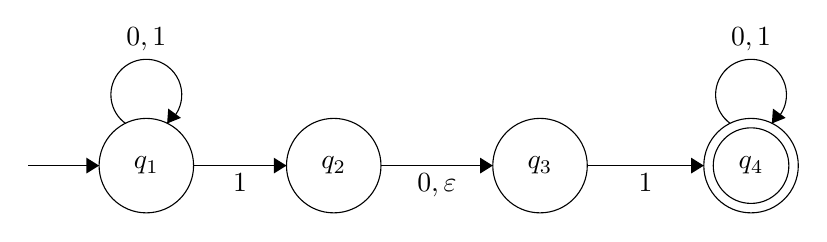
\begin{tikzpicture}[scale=0.2]
        \tikzstyle{every node}+=[inner sep=0pt]
        \draw [black] (15,-24.6) circle (3);
        \draw (15,-24.6) node {$q_1$};
        \draw [black] (26.9,-24.6) circle (3);
        \draw (26.9,-24.6) node {$q_2$};
        \draw [black] (40,-24.6) circle (3);
        \draw (40,-24.6) node {$q_3$};
        \draw [black] (53.4,-24.6) circle (3);
        \draw (53.4,-24.6) node {$q_4$};
        \draw [black] (53.4,-24.6) circle (2.4);
        \draw [black] (7.5,-24.6) -- (12,-24.6);
        \fill [black] (12,-24.6) -- (11.2,-24.1) -- (11.2,-25.1);
        \draw [black] (13.677,-21.92) arc (234:-54:2.25);
        \draw (15,-17.35) node [above] {$0,1$};
        \fill [black] (16.32,-21.92) -- (17.2,-21.57) -- (16.39,-20.98);
        \draw [black] (18,-24.6) -- (23.9,-24.6);
        \fill [black] (23.9,-24.6) -- (23.1,-24.1) -- (23.1,-25.1);
        \draw (20.95,-25.1) node [below] {$1$};
        \draw [black] (29.9,-24.6) -- (37,-24.6);
        \fill [black] (37,-24.6) -- (36.2,-24.1) -- (36.2,-25.1);
        \draw (33.45,-25.1) node [below] {$0,\varepsilon$};
        \draw [black] (43,-24.6) -- (50.4,-24.6);
        \fill [black] (50.4,-24.6) -- (49.6,-24.1) -- (49.6,-25.1);
        \draw (46.7,-25.1) node [below] {$1$};
        \draw [black] (52.077,-21.92) arc (234:-54:2.25);
        \draw (53.4,-17.35) node [above] {$0,1$};
        \fill [black] (54.72,-21.92) -- (55.6,-21.57) -- (54.79,-20.98);
    \end{tikzpicture}
    \caption{A NFA.}
    \label{fig:nfa-1}
\end{figure}

\begin{example}
    Figure \ref{fig:nfa-1} shows a NFA
    which can be described with the regular expression
    \begin{center}
        \ttfamily
        (0|1)*1(0|\textepsilon)1(0|1)*
    \end{center}
    which is equivalent to the regular expression
    \begin{center}
        \ttfamily
        (0|1)*((11)|(101))(0|1)*.
    \end{center}
\end{example}

As you may guess, NFA and DFA are equivalent 
(following from Turing machines),
but we will still put this formally.

\begin{theorem}[Equivalence of DFA and NFA]
    Let $L$ be a formal language.
    Then there exists a DFA $M$ that accepts $L$
    if and only if there exists a NFA $N$ that accepts $L$.
\end{theorem}

From this, we see that a language is regular if a
NFA recognises it too.

\section{B\"uchi automaton}

In our definition, a DFA $M$
may accept a \emph{finite} word $w = w_1 w_2 \ldots w_n$.
We can extend this idea for automaton that may accept
a infinite work $w = w_1 w_2 \ldots$.
We call these kind of machines a \textbf{B\"uchi automaton}.
The formal definition of a B\"uchi automaton $A$ is identical to a
finite-state automaton; however,
$A$ accepts inputs for which there exists $q_f \in F$ which is
infinitely occuring.

\begin{definition}[$\omega$-language]
    An \textbf{$\omega$-language} is a set of infinite length words
    Let $\Sigma$ be a (not necessarily finite) alphabet.
    Then $\Sigma^\omega$ denotes the set of all infinite words over $\Sigma$.
\end{definition}

\begin{definition}[B\"uchi automaton]
    A \textbf{B\"uchi automaton}
    is a $5$-tuple
    \[
        (Q, \Sigma, \delta, q_0, F)
    \]
    defined the same as a DFA;
    however, $M$ accepts a word $w = w_1w_2\ldots \in \Sigma^\omega$
    if there is a sequence of states $(r_0, r_1, \ldots) \in Q^\omega$ satisfying
    \begin{enumerate}
        \item $r_0 = q_0$;
        \item $\delta(r_i, w_{i+1}) = r_{i+1}$ for all $i \in \Z_{\geq0}$; and
        \item there exists an infinitely occuring state which is in $F$.
    \end{enumerate}
    We call $F$ the \emph{acceptance condition}.
\end{definition}

\begin{remark}
    It is clear to see that for an $\omega$-language $L$
    over $\Sigma$ we have $L \subset \Sigma^\omega$.
\end{remark}

We will not define what it means for a B\"uchi automaton
to \emph{recognise} a language, as it is equivalent to
our previous definition.

\begin{definition}[Infinite concatenation]
    Let $A$ be a formal language.
    Then
    \[
        A^\omega = \{a_1a_2\ldots : a_i \in A\}.
    \]
\end{definition}

\begin{definition}[$\omega$-regular language]
    Let $L$ be a $\omega$-language.
    Then $L$ is \textbf{$\omega$-regular} if it has the form
    \begin{enumerate}
        \item $A^\omega$ where $A$ is a non-empty regular language
            with $\varepsilon \not\in A$;
        \item (concatentation) $AB$ 
            where $A$ is a regular language and
            $B$ is a $\omega$-regular language; and
        \item (union) $A \cup B$ 
            where $A,B$ are $\omega$-regular languages
            (this rule can only be applied finitely many times).
    \end{enumerate}
\end{definition}

\begin{theorem}[]
    Let $L$ be an $\omega$-language.
    Then $L$ is \textbf{$\omega$-regular}
    if and only if
    there exists a non-deterministic B\"uchi automaton
    $M$ such that $M$ recognises $L$.
\end{theorem}

\begin{example}[Examples of $\omega$-regular languages]
    \hfill
    \begin{enumerate}
        \item Let $\Sigma = \{0,1\}$.
            Then the following are $\omega$-regular languages:
            \begin{enumerate}
                \item the set of all $\omega$-words
                    containing infinite $0$s; and
                \item the set of all $\omega$-words
                    containing finite $1$s.
            \end{enumerate}
        \item Let $\Sigma = \{0,1,2\}$.
            Then the following are $\omega$-regular languages:
            \begin{enumerate}
                \item the set of all $\omega$-words
                    containing infinitely many $1$s and $2$s
                    but finitely many $0$s;
                \item the set of all $\omega$-words
                    such that after every $1$ there is a $2$; and
                \item the set of all $\omega$-words
                    such that there is an even number of $0$s between pairs
                    of $1$s.
            \end{enumerate}
    \end{enumerate}
\end{example}

\begin{example}
    Consider $L$ to be the $\omega$-language 
    such that each word has a finite number
    of $0$s and an infinite number of $1$s and $2$s.
    We can construct a finite state diagram to construct this diagram.
    \begin{center}
        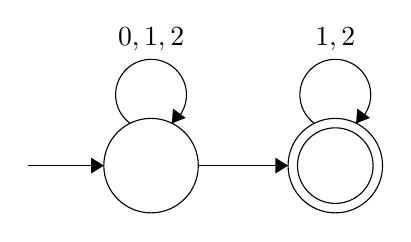
\begin{tikzpicture}[scale=0.2]
            \tikzstyle{every node}+=[inner sep=0pt]
            \draw [black] (13.7,-25.9) circle (3);
            \draw [black] (25.4,-25.9) circle (3);
            \draw [black] (25.4,-25.9) circle (2.4);
            \draw [black] (5.9,-25.9) -- (10.7,-25.9);
            \fill [black] (10.7,-25.9) -- (9.9,-25.4) -- (9.9,-26.4);
            \draw [black] (16.7,-25.9) -- (22.4,-25.9);
            \fill [black] (22.4,-25.9) -- (21.6,-25.4) -- (21.6,-26.4);
            \draw [black] (24.077,-23.22) arc (234:-54:2.25);
            \draw (25.4,-18.65) node [above] {$1,2$};
            \fill [black] (26.72,-23.22) -- (27.6,-22.87) -- (26.79,-22.28);
            \draw [black] (12.377,-23.22) arc (234:-54:2.25);
            \draw (13.7,-18.65) node [above] {$0,1,2$};
            \fill [black] (15.02,-23.22) -- (15.9,-22.87) -- (15.09,-22.28);
        \end{tikzpicture}
    \end{center}
\end{example}

\begin{definition}
    Let $\Sigma$ be an finite alphabet
    and let $A$ be a regular language over $\Sigma$.
    The \textbf{limit} of $A$ is defined as
    \[
        \operatorname{lim}{A} =
        \{a \in \Sigma^w: a \;\text{has infinitely many prefixes in}\;A\}.
    \]
\end{definition}

\begin{example}
    \hfill
    \begin{enumerate}
        \item 
            Consider the regular language over the binary alphabet
            \[
                L = (01)^\star.
            \]
            Then
            \[
                \lim{L} = (01)^\omega.
            \]

        \item 
            Let
            \[
                L = (0 \cup 1)^\star 1.
            \]
            be a regular language over the binary alphabet.
            Let $w \in (0\cup1)^\omega$.
            and $w'$ be an arbitrary prefix of $w$.
            Then $w'1$ is also a prefix of $w$ and $w'1 \in L$.
            So
            \[
                \lim L = (0 \cup 1)^\omega.
            \]
    \end{enumerate}
\end{example}

\begin{theorem}
    An $\omega$-language is a limit of a regular language
    if and only if some deterministic B\"uchi automaton recognises it.
\end{theorem}

\begin{example}
    The language of words consisting of an infinite number of $0$s
    is a limit of a regular language, but the language of words
    consisting of a finite number of $1$s is not.
\end{example}

